\documentclass[% 
%preprint,
final, 
superscriptaddress,
%groupedaddress,
%unsortedaddress,
%runinaddress,
%frontmatterverbose, 
%preprint,
%showpacs,preprintnumbers,
%nofootinbib,
%nobibnotes,
%bibnotes,
 amsmath,amssymb,amsfonts,
 aps,
 pra,
 longbibliography,
%prb,
%rmp,
%prstab,
%prstper,
%floatfix,
]{revtex4-2}

\newcommand{\ket}[1]{\ensuremath{|{#1}\rangle}}
\newcommand{\bra}[1]{\ensuremath{\langle{#1}|}}
\newcommand{\sca}[2]{\ensuremath{\bigl({#1}\cdot{#2}\bigr)}}
\newcommand{\avr}[1]{\ensuremath{\langle{#1}\rangle}}

\newcommand{\cnj}[1]{{#1}^{\ast}}
\newcommand{\hcnj}[1]{{#1}^{\dagger}}
\newcommand{\tcnj}[1]{{#1}^{\mathrm{T}}}

%Differential operators

\newcommand{\prt}[1]{\partial_{#1}}
\newcommand{\pdrs}[1]{\partial_{#1}}
\newcommand{\pdr}[2]{\frac{\partial #1}{\partial #2}}
\newcommand{\drf}[2]{\frac{\dd #1}{\dd #2}}
\newcommand{\vdr}[2]{\dfrac{\delta #1}{\delta #2}}

\newcommand{\ddiv}{\mathop{\rm div}\nolimits}
 \newcommand{\rrot}{\mathop{\rm rot}\nolimits}
 \newcommand{\grad}{\mathop{\rm grad}\nolimits}
\newcommand{\bnbl}{\boldsymbol{\nabla}}

%Functions

\newcommand{\diag}{\mathop{\rm diag}\nolimits}
\newcommand{\sign}{\mathop{\rm sign}\nolimits}
\renewcommand{\Re}{\mathop{\rm Re}\nolimits}
\renewcommand{\Im}{\mathop{\rm Im}\nolimits}
\newcommand{\Tr}{\mathop{\rm Tr}\nolimits}
\newcommand{\ad}{\mathop{\rm ad}\nolimits}
\renewcommand{\ker}{\mathop{\rm Ker}\nolimits}

\newcommand{\cn}{\mathop{\rm cn}\nolimits}
\newcommand{\sn}{\mathop{\rm sn}\nolimits}
\newcommand{\dn}{\mathop{\rm dn}\nolimits}

%Units

\newcommand{\mum}{$\mu$m}
\newcommand{\dega}{$^\circ$}
\newcommand{\degc}{$^\circ$C}
\newcommand{\myarrow}[1]{\ensuremath{\xrightarrow{{#1}^\circ\mathrm{C}}}}

%Symbols

 \newcommand{\bs}[1]{\boldsymbol{#1}}
 \newcommand{\vc}[1]{\mathbf{#1}}
 \newcommand{\mvc}[1]{\mathbf{#1}}
 \newcommand{\uvc}[1]{\hat{\mathbf{#1}}}
 \newcommand{\ubs}[1]{\hat{\boldsymbol{#1}}}
 \newcommand{\ind}[1]{\mathrm{#1}}
\newcommand{\oprt}[1]{\ensuremath{\widehat{\mathcal{#1}}}}

%% 1. Math
\newcommand{\prob}{\mathsf{P}}
\newcommand{\dd}{\mathrm{d}}
\newcommand{\DD}{\ensuremath{\mathcal{D}}}
\newcommand{\JJ}{\ensuremath{\mathcal{J}}}
 \newcommand{\e}{\mathrm{e}}
 \newcommand{\ee}{\mathrm{e}}
\newcommand{\sts}{\ensuremath{\mathcal{Z}}}

\newcommand{\eff}{\mathrm{eff}}
\newcommand{\mx}{\mathrm{max}}
\newcommand{\mn}{\mathrm{min}}

\usepackage[english]{babel}
\usepackage[utf8x]{inputenc}
\usepackage[T1]{fontenc}


%% Useful packages
\usepackage{amsmath}
%\usepackage[colorinlistoftodos]{todonotes}
%\usepackage[colorlinks=true, allcolors=blue]{hyperref}
\usepackage{amssymb,amsmath,amsthm,mathtools,mathrsfs}
\usepackage{graphicx}% Include figure files
\usepackage{multirow}% Include figure files
\usepackage{float}% Include figure files
\usepackage{subcaption}% Include figure files
\usepackage{bbm}

\DeclareMathOperator*{\argmax}{arg\,max}
\DeclareMathOperator*{\argmin}{arg\,min}

%\graphicspath{{figs/}}
\renewcommand{\floatpagefraction}{0.8}

%\selectlanguage{english}

\usepackage{soul,color}
\begin{document}
\DeclareGraphicsExtensions{.png,.pdf}
\title{
  Channel representations of noisy coherent detection in continuous-variable~quantum~key~distribution: Additive-noise versus attenuator
  %Gaussian Channel Parametrization via Coherent Detection Asymmetry and Its Impact on Asymptotic Security of Gaussian Continuous-Variable Quantum Key Distribution in Untrusted Noise Scenario
  %Impact of coherent detection asymmetry effects and channel parameters in untrusted noise continuous variable quantum key distribution
  %Asymmetry effects in untrusted noise securuty analysis
}

\author{A. S.~Naumchik}
\email[Email address: ]{naumchik95@gmail.com}
\affiliation{ITMO University, Kronverksky Pr. 49, Saint Petersburg  197101, Russia}


\author{Roman~K.~Goncharov}
\email[Email address: ]{toloroloe@gmail.com}
\affiliation{ITMO University, Kronverksky Pr. 49, Saint Petersburg  197101, Russia}


\author{Alexei~D.~Kiselev}
\email[Email address: ]{alexei.d.kiselev@gmail.com}
\affiliation{%
  Laboratory for Quantum Communications, ITMO University,
  Birzhevaya Line, 16, Saint Petersburg 199034, Russia}
\affiliation{Laboratory of Quantum Processes and Measurements, ITMO
  University, Kadetskaya Line 3b, Saint Petersburg 199034, Russia} 


\date{\today}

\begin{abstract}
  We study the security of continuous-variable quantum key distribution (CV-QKD) under asymmetric coherent detection within an untrusted-detector model. Building on our previous description of homodyne and double-homodyne receivers, we analyze an attenuator channel and compare it with the additive-noise channel. For both homodyne and double-homodyne detection, we derive the corresponding channel parameters and compare the resulting Holevo information and asymptotic secret fraction.
  
  For the parameter sets considered, receiver asymmetry degrades the protocol performance for both channel models, but neither model gives uniformly more or less pessimistic security estimates. For homodyne detection, the attenuator model gives a lower secret fraction at high transmittance but retains a positive secret fraction over a longer distance.

  In the double-homodyne case, the effects of the ideal Gaussian POVM are proportional to projectors onto displaced squeezed states and depend on the squeezing parameter $r$. The channel parameters and the Holevo information, and hence the resulting secret fraction, depend on $r$, whereas the Alice-Bob mutual information calculated from the calibrated receiver statistics does not.
  For the parameter sets considered, the Holevo information as a function of $r$ is concave for the additive-noise channel and convex for the attenuator channel. It follows that both the choice of $r$ and the channel representation affect the resulting secret fraction.
\end{abstract}
 
 \maketitle

\section{Introduction}
Homodyne and double-homodyne detection are standard coherent measurements in quantum optics and continuous-variable quantum information~\cite{Leonhardt:bk:1997,Weed:rmp:2012,UsenkoRMP2026}. Homodyne detection implements a Gaussian measurement of a single field quadrature, whereas double-homodyne detection performs a joint but necessarily noisy measurement of two conjugate quadratures. In the ideal case, double-homodyne detection realizes the heterodyne POVM. These schemes constitute the measurement stage in a broad range of continuous-variable quantum communication, including protocols for continuous-variable quantum key distribution (CV-QKD)~\cite{Weedbrook:prl:2004,
   Pirandola:advopt:2020}, quantum state tomography~\cite{d2003quantum, Lvovsky:rmp:2009}, and quantum state preparation~\cite{Zhang_2019}.

Practical coherent receivers are affected by beam-splitter imbalance
and by nonunit and generally unequal quantum efficiencies of the photodetectors. These imperfections modify the conditional distribution of Bob's
outcomes and can bias the security estimate when omitted from the
measurement model~\cite{Pereira:epjqt:2021,Mi2024BiasedDetection,
hajomer2025finite}. The receiver model retains these nonunit efficiencies, whereas receiver asymmetry refers specifically
to beam-splitter imbalance and efficiency mismatch between the detection branches. Assuming
the strong local oscillator, they are
described by noisy Gaussian POVMs. Electronic noise, finite detector
range and resolution, and active detector imperfections are distinct
effects and are not part of the asymmetry model derived here.

For each noisy Gaussian measurement considered here, the measurement statistics can be represented by applying a Gaussian channel
to the incoming mode before an ideal Gaussian measurement or,
equivalently, by applying its dual channel to the ideal measurement
operators~\cite{HolevoGaussianObservable2021,Serafini:bk:2023}.
An invertible deterministic rescaling of the outcomes is included when matching the resulting measurement statistics to those of the physical receiver. This representation is particularly useful in CV-QKD because it incorporates receiver imperfections into the same formalism used to describe the transformation of quantum states by the communication channel and to evaluate the information available to an eavesdropper. Two natural Gaussian channels are the additive-noise channel and the attenuator channel. The former applies a random displacement sampled from a zero-mean Gaussian distribution, with displacement quadratures uncorrelated with the input quadratures, whereas the latter mixes the input mode with an environmental mode at a beam splitter. The attenuator reduces to a pure-loss channel when the environmental mode is in the vacuum state~\cite{HolevoGaussianChannels2007,CarusoGaussianChannels2006}. With suitable channel parameters, the two channels reproduce the same conditional outcome distributions after the outcome rescaling.

Equivalence at the level of measurement statistics does not, however, imply equivalence as a
quantum measurement process. A POVM fixes the outcome probabilities
but does not by itself fix the corresponding quantum information transferred to unobserved degrees of freedom
~\cite{DaviesLewis1970,Holevo1973Statistical,Ozawa1984}. Using a particular channel representation in the security analysis introduces an additional physical assumption whose interpretation depends on whether receiver noise is trusted. In a trusted-detector model, the degrees of freedom associated with calibrated
receiver noise remain inside Bob's laboratory~\cite{Lodewyck:pra:2007,Usenko:entropy:2016,Laudenbach:aqt:2018,Laudenbach:aqt:2019,Namiki2018DetectionChannel}. In the
untrusted-detector model adopted here, the environmental output
of the selected channel is assigned to Eve. Different
channels may then give the same calibrated receiver
statistics and the same mutual information while producing different Alice-Bob states, different environmental outputs, and different values of the Holevo information. More recent works refine this dichotomy by considering several levels of trust for loss and noise and by separating Eve's knowledge of detector noise from her ability to control it~\cite{PirandolaTrustLevels2021,Pan:pra:2025,Zuo2026ThreatModels}.
Purification of a fixed state is related by an
isometry on the purifying system~\cite{Nielsen:bk:2010}. Here, applying the alternative
channels to the incoming state produces different Alice-Bob states before the ideal
measurement. Selecting a particular channel representation therefore introduces a physical
assumption about the coupling of the optical signal to inaccessible
degrees of freedom.

Representing calibrated detector noise as an effective loss has
previously been used in trusted and protocol-specific receiver models
~\cite{Zhang2020OneTimeCalibration,Zou:optexp:2022,
Yamano2023GaussianTrustedNoise,Wu2026OneTimeCalibration}. Such equivalence at the level of receiver statistics does not by itself determine
whether the corresponding environmental mode is accessible to Eve.

In our previous work~\cite{naumchik2025asymmetryeffectshomodyneheterodyne}, we derived the Gaussian POVMs that account for beam-splitter imbalance and photodetector efficiency mismatch, collectively referred to as \textit{asymmetry effects} in coherent receivers. We represented the resulting measurement noise through an additive-noise channel. For double-homodyne detection, the effects of the ideal Gaussian POVM were proportional to projectors onto displaced squeezed states and depended on the squeezing parameter $r$. The admissible interval of squeezing parameters was fixed by the positivity of the excess-noise covariance matrix. When the environmental output of the channel is assigned to Eve, different admissible values of $r$ yield different values of the Holevo information, although the noisy POVM remains fixed. Although mathematically straightforward, the additive-noise channel is not tied to a specific optical coupling mechanism and is not the only channel compatible with the same noisy POVM. This leaves open how the security estimate changes between Gaussian channels compatible with the same noisy POVM.

In the present work, we construct an attenuator channel that reproduces the calibrated receiver statistics of the asymmetric homodyne and double-homodyne POVMs and compare it with the additive-noise channel. The channel parameters are obtained by requiring the dual channel, together with an invertible deterministic rescaling of the outcomes, to reproduce the measurement statistics of the target noisy POVM. For homodyne detection, the environmental mode is chosen to be in the vacuum state, so the attenuator takes the form of a pure-loss channel. For double-homodyne detection, the generally anisotropic measurement noise is reproduced using a pure Gaussian state of the environmental mode with generally unequal quadrature variances. The channels considered here therefore serve as representations of a fixed noisy measurement rather than as alternatives to the physical communication channel.

We compare the two channels within the Gaussian-modulated coherent-state (GMCS) CV-QKD protocol~\cite{Grosshans:prl:2002,GrosshansNature2003} with reverse reconciliation in the asymptotic regime and evaluate the asymptotic secret fraction under collective Gaussian attacks~\cite{Miguel:prl:2006,Cerf:prl:2006}. The GMCS protocol provides a natural setting for a direct covariance-matrix comparison of the two models. The receiver imperfections are treated within an untrusted-detector model, so the environmental output of the selected
channel is assigned to Eve.
The comparison is restricted to the additive-noise channel and to attenuator channels whose environmental modes are in pure Gaussian states. The reported secret fractions are therefore conditional on the chosen channel representation. Finite-size effects, composable-security corrections, mixed environmental states, active detector attacks, and uncertainties in equipment calibration are
outside the present scope.

The paper is organized as follows. Section~\ref{sec:POVMs} summarizes
the asymmetric homodyne and double-homodyne Gaussian POVMs derived in
Ref.~\cite{naumchik2025asymmetryeffectshomodyneheterodyne}.
Section~\ref{sec:channels} constructs the additive-noise and attenuator
channels and derives their
parameters. Section~\ref{sec:protocol} evaluates the mutual information,
the Holevo information, and the asymptotic secret
fraction and compares the two channels. Finally,
Sec.~\ref{sec:conclusion} discusses the physical interpretation,
limitations, and security implications of the results.

\section{Imperfect Gaussian measurements}\label{sec:POVMs}
We begin with a brief discussion of asymmetrical coherent measurements, schematically depicted in Fig.~\ref{fig:scheme}. Asymmetry effects are induced by imbalance (unequal transmission and reflection coefficients) of the beam splitters and unequal quantum efficiency of the detectors. For detailed derivations of the expressions in this section see Ref.~\cite{naumchik2025asymmetryeffectshomodyneheterodyne}.

$Q$ symbol of the POVM describing noisy homodyne measurements (see Fig.~\ref{subfig:homodyne}) is given by
\begin{align}
  &\label{eq:Pgood-w-def}
    {\prob}_G^{(\ind{H})}(x)=\frac{1}{\sqrt{2\pi\sigma_G}}
    \exp \left[-\frac{(x-\avr{\hat{x}_\phi})^2}{2\sigma_x}\right],\\
  &\label{eq:avr-x-phi}
  \avr{\hat{x}_\phi}\equiv \bra{\alpha}\hat{x}_\phi\ket{\alpha}={2\Re\alpha e^{-i\phi}},
  \quad \phi=\arg\alpha_L,\\
    &\label{eq:quad-op}
    \hat{x}_\phi=\hat{a}e^{-i\phi}+\hat{a}^\dag e^{i\phi}
\end{align}
where $\alpha$ ($\alpha_L$) is the complex amplitude of signal (LO) mode, $\hat{x}_\phi$ is the phase-rotated quadrature operator;
$x$ is the quadrature variable
\begin{align}
  \label{eq:x-def}
  x\equiv\frac{\mu}{(\eta_1+\eta_2)CS\left|\alpha_L\right|}-\frac{\eta_1S^2-\eta_2C^2}{\left(\eta_1+\eta_2\right)CS}\left|\alpha_L\right|
\end{align}
and $\sigma_x$ is the quadrature variance
\begin{align}
  &
        \label{eq:sigma-x}
    \sigma_x\equiv
    \frac{\eta_1S^2+\eta_2C^2}{
    \left[(\eta_1+\eta_2)CS\right]^2
    }.
\end{align}

By computing inverse Forier transform of $Q$ symbol~\eqref{eq:Pgood-w-def}, we obtain anti-normal ordered characteristic function~\cite{Serafini:bk:2023}. From this characteristic function we can deduce the covariance matrix of the noisy homodyne measurements as follows %(see also Ref.~\cite{naumchik2025asymmetryeffectshomodyneheterodyne} for derivation)
\begin{align}
    &\label{eq:Sigma-H-m}
    \Sigma_{m}^{(\ind{H})}= \lim_{r\to+\infty}R(\phi)\,\ind{diag}(e^{-2r}+\sigma_N,e^{2r})\,\tcnj{R}(\phi)
    %=\Sigma_{\ind{id}}^{(\ind{H})}+\Sigma_{N}^{(\ind{H})}
    ,\\
    &\label{eq:Sigma-H-id}
    \Sigma_{\ind{id}}^{(\ind{H})}=\lim_{r\to+\infty}R(\phi)\,\ind{diag}(e^{-2r},e^{2r})\,{R}^{\ind{T}}(\phi)%\\
    %&\label{eq:Sigma-N-H}
    %\Sigma_{N}^{(\ind{H})}=R(\phi)\,\ind{diag}(\sigma_N,0)\,\tcnj{R}(\phi)
    ,
\end{align}
where $\Sigma_{\ind{id}}^{(\ind{H})}$ is the covariance matrix of ideal homodyne measurement, $R(\phi)=\begin{pmatrix}\cos\phi&-\sin\phi\\ \sin\phi& \cos\phi\end{pmatrix}$ is the rotation matrix; $\sigma_N$ is the excess noise variance that accounts for asymmetry effects is given by
\begin{align}
  &
  \label{eq:sgm_N}
     \sigma_N=\sigma_x-1.
\end{align}

\begin{figure}
    \centering
    \begin{subfigure}[c]{.45\linewidth}
      \centering
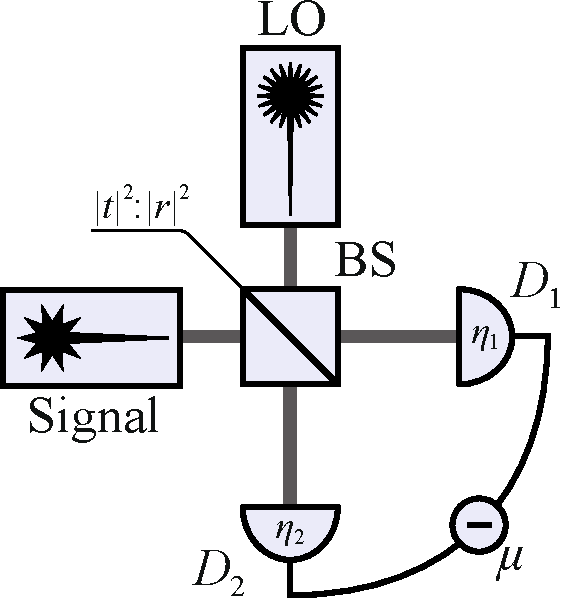
\includegraphics[height= .3\textheight]{schemes/homodyne.pdf}
\caption[]{}
\label{subfig:homodyne}
    \end{subfigure}
    \hfill
    \begin{subfigure}[c]{.45\linewidth}
      \centering
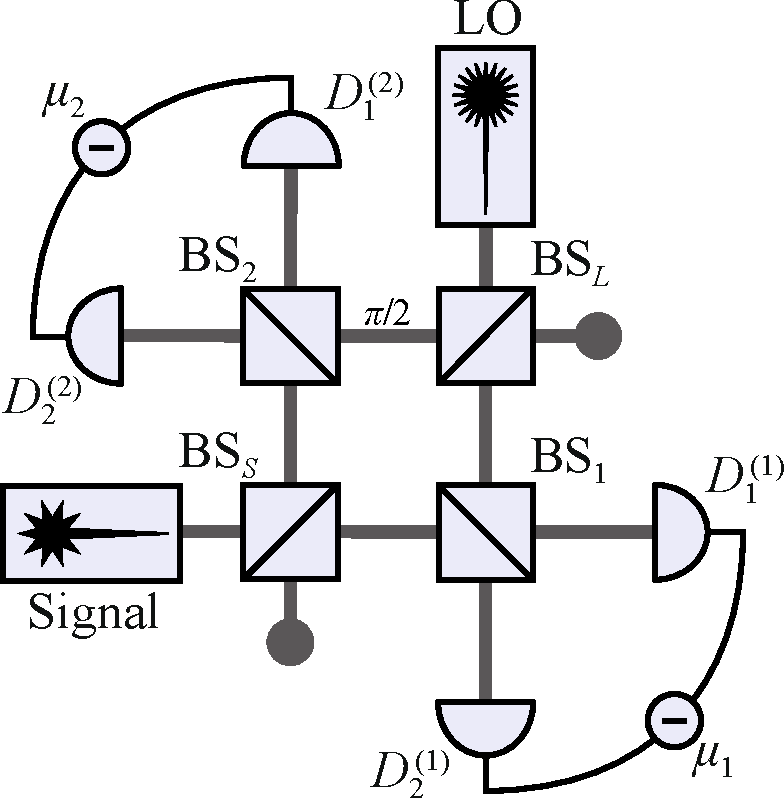
\includegraphics[height= .3\textheight]{schemes/double-homodyne.pdf}
\caption[]{}
\label{subfig:double-homodyne}
    \end{subfigure}
 \caption[]{
  (a)~Scheme of homodyne receiver. S (LO) is the source of signal (reference) mode, BS is the beam splitter with transmission and
  reflection coefficients $C$ and $S$, respectively; photodetectors $D_1$ and $D_2$ have quantum efficiencies $\eta_1$ and $\eta_2$, and $\mu=m_1-m_2$ is the photon count difference.
  (b)~Scheme of double-homodyne receiver. S (LO) is the source of signal (reference) mode, BS$_S$ (BS$_L$) is the signal mode (local oscillator) beam splitter; $\frac{\pi}{2}$ is the quarter wave phase shifter; BS$_i$ is the beam splitter of $i$th homodyne; $D_{1,2}^{(i)}$ are the photodetectors of the $i$th homodyne; and $\mu_i=m_1^{(i)}-m_2^{(i)}$ is the photon count difference registered by the detectors of $i$th homodyne.}
  \label{fig:scheme}
\end{figure}

For double-homodyne detection, $Q$ symbol is given by
\begin{align}
  \label{eq:P_G-x1x2}
  &
    \prob_G^{(\ind{DH})}(x_1,x_2)
    =\frac{1}{2\pi\sqrt{\sigma_G^{(1)}\sigma_G^{(2)}}}
    \exp\biggl[
    -\frac{(x_1-\Re\alpha e^{-i\phi})^2}{\sigma_1}
    -\frac{(x_2-\Im\alpha e^{-i\phi})^2}{\sigma_2}
    \biggr],\\
    &
    \label{eq:sigma_G-i}
    \sigma_G^{(i)}=
    (\eta_1^{(i)}S_i^2+\eta_2^{(i)}C_i^2) |\alpha_L^{(i)}|^2,\quad
    \alpha_L^{(1)}=C_L\alpha_L,\quad \alpha_L^{(2)}=-iS_L\alpha_L,
\end{align}
where $x_i$ are the quadrature variables given by
\begin{align}
  \label{eq:x-1}
  x_1&=
  \frac{1}{2(\eta_1^{(1)}+\eta_2^{(1)})C_1S_1C_S}
  \left\{
  \frac{\mu_1}{|\alpha_L^{(1)}|}-(\eta_1^{(1)}S_1^2-\eta_2^{(1)}C_1^2) |\alpha_L^{(1)}|
    \right\},
  \\
  \label{eq:x-2}
  x_2&=
  \frac{1}{2(\eta_1^{(2)}+\eta_2^{(2)})C_2S_2S_S}
  \left\{
  \frac{\mu_2}{|\alpha_L^{(2)}|}-(\eta_1^{(2)}S_2^2-\eta_2^{(2)}C_2^2) |\alpha_L^{(2)}|
    \right\},
\end{align}
and relations
\begin{align}
  &
  \label{eq:sigm-i}
    \sigma_1=\frac{\sigma_x^{(1)}}{ 2 C_S^2},
    \quad
    \sigma_2=\frac{\sigma_x^{(2)}}{ 2 S_S^2},
  \\
  &
    \label{eq:sigm-x-i}
    \sigma_x^{(i)}=\frac{\eta_1^{(i)}S_i^2+\eta_2^{(i)}C_i^2}{
    \left[(\eta_1^{(i)}+\eta_2^{(i)})C_iS_i\right]^2
    }
\end{align}
give the quadrature variances $\sigma_1$ and $\sigma_2$.

Following the same procedure used to derive Eq.~\eqref{eq:Sigma-H-m}, we obtain the covariance matrix of the double-homodyne POVM,
\begin{align}
\label{eq:Sigma_m-DH}
  &
  \Sigma_m^{(\ind{DH})}=R(\phi)\diag(\delta_1,\delta_2)\tcnj{R}(\phi),
  \\
  \label{eq:sigma-i}
  &
    \delta_i=2\sigma_i-1.
\end{align}

The POVM that describes ideal double-homodyne measurements uses the set of squeezed states,
\begin{align}
  \label{eq:squeezed-def}
  \ket{z,r,\phi}=\hat{R}(\phi)\hat{D}(z)\hat{S}(r)\ket{0}=
  \hat{D}(z e^{i\phi})\hat{S}(r e ^{2i\phi})\ket{0},
\end{align}
where $z$ is the coherent state amplitude, $r$ is real-valued squeezing parameter, and $\phi$ is squeezing phase,
$\hat{D}(z) =
e^{z\hcnj{\hat{a}}-z^*\hat{a}}$ is the displacement operator, and $\hat{S}(r)=e^{\frac{1}{2}\left(r\hat{a}^{\dag2}-r^*\hat{a}^2\right)}$ is the squeezing operator.

The covariance matrix of squeezed states reads
\begin{align}
  \label{eq:Sigma-id-DH}
  &
  \Sigma_{\ind{id}}^{(\ind{DH})}=
    R(\phi)
    \begin{pmatrix}
      e^{2r}&0\\0&e^{-2r}
    \end{pmatrix}
    \tcnj{R}(\phi).
\end{align}

An important point is that, for the difference between comvariance matrices of noisy and ideal double-homodyne measurements, given by Eq.~\eqref{eq:Sigma_m-DH} and Eq.~~\eqref{eq:Sigma-id-DH} respectively, is positive semi-definite, the squeezing parameter $r$ must be ranged in the interval defined by parameters of the scheme (see Ref.~\cite{naumchik2025asymmetryeffectshomodyneheterodyne})
\begin{align}
  \label{eq:r1-r2}
  &
    r\in \left[r_2,r_1\right],\;
    r_1=\ln\delta_1^{1/2},
    \;
    r_2=\ln\delta_2^{-1/2}.
\end{align}

\section{Gaussian channels modeling imperfect measurements}\label{sec:channels}
For arbitrary state $\hat{\rho}$ and POVM ${\hat{\Pi}^{(x)}}$, the outcome probability is~\cite{Nielsen:bk:2010}
\begin{align}
p(x|\hat{\rho})=\Tr\left(\hat{\rho}\,\hat{\Pi}^{(x)}\right).
\end{align}

The measurement statistics of Gaussian states with noisy Gaussian measurements can be calculated by applying the noise map $\mathcal{C}$ to $\rho_G$, or the dual map $\mathcal{C}^*$ to the ideal POVM $\hat{\Pi}_{\ind{id}}$~\cite{Serafini:bk:2023}, i.e.
\begin{align}
  \label{eq:channel-motiv}
  p(x|\hat\rho_G)=\Tr\left\{\mathcal{C}(\hat\rho_G)\,\hat\Pi_{\ind{id}}^{(x)}\right\}
  =\Tr\left\{\hat\rho_G\,\mathcal{C}^{*}\left(\hat\Pi_{\ind{id}}^{(x)}\right)\right\}.
\end{align}

For the measurements considered here, different Gaussian channels $\mathcal{C}$ can reproduce the same measurement statistics after an invertible deterministic rescaling of the outcomes. The channel parameters are chosen so that their dual maps $\mathcal{C}^{*}$ generate the same measurement covariance matrix, while the rescaling aligns the first moments.

We consider only Gaussian channels $\mathcal{C}$ with zero displacement. Such a channel is fully characterized by matrices $X_{\mathcal{C}}$ and $Y_{\mathcal{C}}$, which transform the first and second moments of the Gaussian state $\rho_G$, $\boldsymbol{r}_G$ and $\Sigma_G$, respectively, as follows~\cite{Weed:rmp:2012}:

\begin{align}
  &\boldsymbol{r}_G\mapsto X_{\mathcal{C}}\boldsymbol{r}_G,\notag\\
  \label{eq:X,Y-action}
  &\Sigma_G\mapsto X_{\mathcal{C}}\Sigma_G X_{\mathcal{C}}^{\ind{T}}+Y_{\mathcal{C}}.
\end{align}

The dual channel $\mathcal{C}^*$ transforms the first and second moments as follows:
\begin{align}
  &\boldsymbol{r}_G\mapsto X_{\mathcal{C}}^{-1}\boldsymbol{r}_G,\notag\\
  &\Sigma_{G}\mapsto  X_{\mathcal{C}}^{-1}\Sigma \left({X_{\mathcal{C}}^{-1}}\right)^{\ind{T}}+X_{\mathcal{C}}^{-1}Y_{\mathcal{C}}\left({X_{\mathcal{C}}^{-1}}\right)^{\ind{T}}.
\end{align}

In what follows, we will consider two distinct quantum channels to describe the imperfect measurements, namely the additive-noise channel and the attenuator channel. In accordance with Eq.~\eqref{eq:channel-motiv}, channel $\mathcal{C}$ will be defined so that its dual channel $\mathcal{C}^*$ transforms the covariance matrix of the ideal measurement $\Sigma_{\ind{id}}$ into the covariance matrix of the noisy Gaussian measurement $\Sigma_{m}$,
\begin{align}
  \label{eq:C-gen}
  \mathcal{C}^*:\quad \Sigma_{\ind{id}}^{(\gamma)}\mapsto\Sigma_{m}^{(\gamma)}
\end{align}

\subsection{Additive-noise channel}
First, we consider additive-noise (classical mixing) channel~\cite{Serafini:bk:2023} $\Phi_{\gamma}$, characterized by matrices
\begin{align}
    \label{eq:X,Y-phi}
    X_{\Phi}^{(\gamma)}=\mathbbm{1}, \quad Y_{\Phi}^{(\gamma)}\geq0, \quad \gamma\in\{\ind{H}, \ind{DH}\}.
\end{align}
This is a self-dual channel,
$\cnj{\Phi}_\gamma=\Phi_\gamma$, that does not affect the first moment and changes the second moment as follows
\begin{align}
  \Phi_\gamma:
  \Sigma\mapsto
  \Sigma+Y_{\Phi}^{(\gamma)}.
\end{align}

To find matrices $Y_{\Phi}^{(\gamma)}$ so that (see Eq.~\eqref{eq:C-gen})
\begin{align}
  \label{eq:add-act}
  \Phi_{\gamma}:\quad \Sigma_{\ind{id}}^{(\gamma)}\mapsto\Sigma_m^{(\gamma)}=\Sigma_{\ind{id}}^{(\gamma)}+Y_{\Phi}^{(\gamma)},
\end{align}
we need to find the difference between covariance matrices of noisy and ideal measurements, i.e.
\begin{align}
  Y_{\Phi}^{(\gamma)}=\Sigma_{m}^{(\gamma)}-\Sigma_{\ind{id}}^{(\gamma)}\equiv \Sigma_{N}^{(\gamma)},
\end{align}
where we defined the covariance matrix of excess noise $\Sigma_{N}^{(\gamma)}$.

For homodyne detection, from Eq.~\eqref{eq:Sigma-H-id} and~\eqref{eq:Sigma-H-m}, we have
\begin{align}
    &
    \label{eq:Sigma-N-H}
    \Sigma_{N}^{(\ind{H})}=
    \Sigma_{m}^{(\ind{H})}-\Sigma_{\ind{id}}^{(\ind{H})}= R(\phi)
    \ind{diag}(\sigma_N, 0)
    \tcnj{R}(\phi)\ge 0,
\end{align}
where $\sigma_N$ is given by Eq.~\eqref{eq:sgm_N}.

For double-homodyne detection, from Eq.~\eqref{eq:Sigma_m-DH} and~\eqref{eq:Sigma-id-DH}, we have
\begin{align}
  &
    \label{eq:Sigma-N-DH}
    \Sigma_{N}^{(\ind{DH})}(r)=
    \Sigma_{m}^{(\ind{DH})}-\Sigma_{\ind{id}}^{(\ind{DH})}= R(\phi)
\begin{pmatrix}
      \sigma_N^{(1)}(r) &0\\0&\sigma_N^{(2)}(r)
    \end{pmatrix}
    \tcnj{R}(\phi)\ge 0,\\
  \label{eq:sigma_N-sq-2}
  &
    \sigma_N^{(1)}(r)=\delta_1-e^{2r},
    \quad
    \sigma_N^{(2)}(r)=\delta_2-e^{-2r}.
\end{align}
Note that the elements of $\Sigma_{N}^{(\ind{DH})}$ are dependent on squeezing parameter that lies in the interval~\eqref{eq:r1-r2}. When $r\in[r_2,r_1]$, it is certain that the covariance matrix of excess noise is positive semi-definite, $\Sigma_{N}^{(\ind{DH})}(r)\geq0$.

\subsection{Attenuator channel}
We shall move on to the attenuator channel $\mathcal{E}_{\gamma}$,
characterized by matrices~\cite{Serafini:bk:2023}
\begin{align}
    \label{eq:X,Y}
    X_{\mathcal{E}}^{(\gamma)}=\cos\theta_{\gamma}\mathbbm{1}, \quad Y_{\mathcal{E}}^{(\gamma)}=\sin^2\theta_{\gamma}\Sigma_{\ind{env}}^{(\gamma)}, \quad \gamma \in \{\ind{H}, \ind{DH}\},
\end{align}
where $\Sigma_{\ind{env}}^{(\gamma)}$ is the covariance matrix of the state decribing the enviroment.

Using Eq.~\eqref{eq:C-gen} together with Eq.~\eqref{eq:X,Y-action}, we construct the dual channel $\mathcal{E}_N^{*(\gamma)}$ so that it transforms the POVM of the ideal measurement into the POVM of the noisy measurements by changing the covariance matrix $\Sigma_{\ind{id}}^{(\gamma)}$ into $\Sigma_{m}^{(\gamma)}$ as follows
\begin{align}
    \label{eq:psi_ast}
    \mathcal{E}_{\gamma}^{*}:\quad \Sigma_{\ind{id}}^{(\gamma)}\mapsto\Sigma_{m}^{(\gamma)}=\frac{1}{\cos^2\theta_{\gamma}}\Sigma_{\ind{id}}^{(\gamma)}+\tan^2\theta_{\gamma}\Sigma_{\ind{env}}^{(\gamma)},
    \quad \gamma\in\{\ind{H},\ind{DH}\}.
\end{align}

First, we will consider homodyne detection. If the enviroment is decribed by vacuum, i.e.
\begin{align}
    \label{eq:sigma-anc-h}
    \Sigma_{\ind{env}}^{(\ind{H})}=\mathbbm{1},
\end{align}
together with from matrices of ideal~\eqref{eq:Sigma-H-id} and noisy~\eqref{eq:Sigma-H-m} measurements, Eq.~\eqref{eq:psi_ast} takes the form
\begin{align}
  \Sigma_{m}^{(\ind{H})}=\lim_{r\to+\infty}R(\phi)\,\ind{diag}(e^{-2r}+\sigma_N,e^{2r})\,\tcnj{R}(\phi)=\lim_{r\to+\infty}\left\{
    \frac{1}{\cos^2\theta_{\ind{H}}}R(\phi)\,\ind{diag}(e^{-2r},e^{2r})\,{R}^{\ind{T}}(\phi)
    +
    \tan^2\theta_{\ind{H}}\mathbbm{1}
    \right\}
\end{align}
due to the limit $r\to\infty$, we may write
\begin{align}
    &\frac{1}{\cos^2\theta}\Sigma_{\ind{id}}^{(\ind{H})}\sim
    \Sigma_{\ind{id}}^{(\ind{H})}, \quad e^{2r}+\ind{const}\sim e^{2r},
\end{align}
it is sufficient to solve for $\tan^2\theta_{\ind{H}}$, i.e.
\begin{align}
  \label{eq:tan2theta-h}
  \tan^2\theta_{\ind{H}}=\sigma_N, %\quad\Sigma_{\mathcal{E}_{\ind{H}}}\equiv R(\phi)\,\ind{diag}(\sigma_N,\sigma_N)\,{R}^{\ind{T}}(\phi).
\end{align}
where $\sigma_N$ is defined by Eq.~\eqref{eq:sgm_N}. Then, $\cos^2\theta_{\ind{H}}$ and $\sin^2\theta_{\ind{H}}$ are given by
\begin{align}
    \label{eq:cos-theta-h}
    &\cos^2\theta_{\ind{H}}={\frac{1}{\sigma_x}},\quad
    \sin^2\theta_{\ind{H}}={\frac{\sigma_N}{\sigma_x}}.
\end{align}

For double-homodyne detection with $\delta_1\neq\delta_2$, the environmental state obtained below is generally anisotropic for an arbitrary admissible value of $r$, although it can be isotropic at a special value of $r$. In the attenuator channel model studied here, we restrict the environmental mode to a pure state with $\det\Sigma_{\ind{env}}^{(\ind{DH})}=1$,
\begin{align}
  \label{eq:anc-dh-def}
    \Sigma_{\ind{env}}^{(\ind{DH})}=R(\phi)\,\ind{diag}\left(a,\frac1a\right)\,{R}^{\ind{T}}(\phi),\quad a>0.
\end{align}
Solving Eq.~\eqref{eq:psi_ast} for the case of double-homodyne detection, (see Eq.~\eqref{eq:Sigma-id-DH},~\eqref{eq:Sigma_m-DH}),
\begin{align}
  \Sigma_{m}^{(\ind{DH})}=
  R(\phi)\diag(\delta_1,\delta_2)\tcnj{R}(\phi)
  =R(\phi)\,\left\{
    \frac{1}{\cos^2\theta_{\ind{DH}}}\,\ind{diag}(e^{2r},e^{-2r})
    +
    \tan^2\theta_{\ind{DH}}\,\ind{diag}\left(a,\frac{1}{a}\right)
    \right\}\,{R}^{\ind{T}}(\phi),
\end{align}
\begin{align}
    \label{eq:system-dh}
    \begin{cases}
        \delta_1=\frac{e^{2r}}{\cos^2\theta_{\ind{DH}}}+\tan^2\theta_{\ind{DH}} a\\
        \delta_2=\frac{e^{-2r}}{\cos^2\theta_{\ind{DH}}}+\tan^2\theta_{\ind{DH}} a^{-1}
    \end{cases}.
  \end{align}
Solving the system yields
\begin{align}
    \label{eq:cos-theta-dh}
    &\cos^2\theta_{\ind{DH}}(r)={\frac{e^{2r}+a(r)}{\delta_1+a(r)}}=
    \frac{\delta_1 e^{-2r}+\delta_2e^{2r}-2}{\delta_1\delta_2-1}
    ,\\
    \label{eq:a_def}
    &a(r)=\frac{\delta_{1}-e^{2 r}}{\delta_{2} e^{2 r}-1}.%\frac{1}{2}\left[-b+ \sqrt{b^2-4c}\right],\quad
    %b=\frac{-\delta_1e^{-2r}+\delta_2e^{2r}}{\sigma_N^{(2)}},\quad c=\frac{-\sigma_N^{(1)}}{\sigma_N^{(2)}}
    %,\\
    %&\sigma_N^{(1)}=\delta_1-e^{2r}, \quad \sigma_N^{(2)}=\delta_2-e^{-2r}.
\end{align}

Note that at the ends of the $r$-interval~\eqref{eq:r1-r2}, $r\to r_2$ or $r\to r_1$, either $a(r)$ or $1/a(r)$ tend to infinity, making the ancilla state~\eqref{eq:anc-dh-def} the eigenstate of the quadrature operator~\eqref{eq:quad-op}. By evaluating in this case the equations~\eqref{eq:system-dh}, i.e. resolving indeterminate form $\tan^2\theta_{\ind{DH}} a(r)$ for $r=r_2$ and $\tan^2\theta_{\ind{DH}}/a(r)$ for $r=r_1$, because one of noise variances~\eqref{eq:sigma_N-sq-2} would be $0$, it can be seen that the effect of this channel would be the same as the effect of the additive-noise channel~\eqref{eq:add-act} modeling double-homodyne detection with the same $r$. This fact will be used in numerical calculations (see next section and Fig.~\ref{fig:Entropy}).

\section{Gaussian-modulated coherent-state protocol}\label{sec:protocol}
In the Gaussian-modulated coherent-state (GMCS) protocol, Alice samples the complex amplitude $\alpha=\alpha_1+i\alpha_2$ from the Gaussian prior:
\begin{align}
  p_A(\alpha)
  =\frac{1}{\pi V_{\ind{A}}}\exp\!\left[-\frac{|\alpha|^2}{2V_{\ind{A}}}\right].
\end{align}
She then prepares the coherent state $\ket{\alpha}$.
The states pass the composite Gaussian channel $\mathcal{N}_{A\to B}=\mathcal{L}_{N}\circ\mathcal{L}_{T_{\ind{ch}}}$, where index indicates pure loss channel transmission coefficient, $T_{\ind{ch}}$ is the channel transmittance, $N=1+\xi_{\ind{ch}}/(1-T_{\ind{ch}})$, and $\xi_{\ind{ch}}$ is the channel excess noise.
Then, the receiver uses either homodyne or double-homodyne detection to measure the states. Mutual information between legitimate parties in each case is then given by the following expressions (see Ref.~\cite{naumchik2025asymmetryeffectshomodyneheterodyne} for derivation)
\begin{align}
  \label{eq:I_H_res}
  &I_{\ind{AB}}^{(\ind{H})}=\frac{1}{2}\log\left[1+\frac{4T_{\ind{ch}}V_{\ind{A}}}{\sigma_x+\xi_{\ind{ch}}}\right],\\
  \label{eq:I_DH_res}
  &I_{\ind{AB}}^{(\ind{DH})}=\frac{1}{2}\sum_i\log\left[1+\frac{4T_{\ind{ch}}V_{\ind{A}}}
    {2 \sigma_i+\xi_{\ind{ch}}}\right],
\end{align}
where $\sigma_x$ and $\sigma_i$ given by Eqs.~\eqref{eq:sigma-x} and~\eqref{eq:sigm-x-i}, respectively, and upper indices hereinafter stand for homodyne and double-homodyne detection.

The covariance matrix of TMSV state with the Bob's mode
transmitted through the noisy channel reads
(see Ref.~\cite{Laudenbach:aqt:2018})
\begin{align}
  \label{eq:TMSVS-to-AB}
  \mathcal{I}_A&\otimes \mathcal{L}_{N}\circ\mathcal{L}_{T_{\ind{ch}}}:
\quad
    \Sigma_{\ind{TMSV}}
  =
  \begin{pmatrix}
        V\mathbbm{1}&\sqrt{V^2-1}\sigma_z\\
        \sqrt{V^2-1}\sigma_z&V\mathbbm{1}
    \end{pmatrix}
  \mapsto
    \Sigma_{\ind{AB}}
    =
    \begin{pmatrix}
        V\mathbbm{1}&c\sigma_z\\
        c\sigma_z&V_{\ind{B}}\mathbbm{1}
    \end{pmatrix},
\end{align}
where
$\mathcal{I}_A$ is the identity channel acting on the subsystem $A$
and the parameters of the covariance matrix
$\Sigma_{\ind{AB}}$ are given by
\begin{align}
  \label{eq:V-c}
  &
    V=1+4V_{\ind{A}},
    \quad c=\sqrt{T_{\ind{ch}}(V^2-1)},
  \\
  &
  \label{eq:V_B}
    V_{\ind{B}}=T_{\ind{ch}}(V-1)+1+\xi_{\ind{ch}}.
\end{align}


We consider local action of either attenuator channel $\mathcal{E}_{\gamma}$~\eqref{eq:X,Y} or additive-noise channel $\Phi_{\gamma}$~\eqref{eq:X,Y-phi}, on second mode of TMSVS shared by Alice and Bob~\eqref{eq:TMSVS-to-AB}. In both cases, mutual information is given by $I_{\ind{AB}}^{(\gamma)}$~\eqref{eq:I_H_res},~\eqref{eq:I_DH_res}, as it is classical.

It follows
\begin{align}
    \label{eq:psi_action}
    &\mathcal{I}_A\otimes \mathcal{E}_{\gamma}:
    \Sigma_{\ind{AB}}\mapsto
     \Sigma_{\ind{AB}}^{(\mathcal{E}_{\gamma})}
     =\begin{pmatrix}
        V\mathbbm{1}&c\cos\theta_{\gamma}\sigma_z\\
     c\cos\theta_{\gamma}\sigma_z&\cos^2\theta_{\gamma}
     \left(V_{\ind{B}}+\tan^2\theta_{\gamma}\Sigma_{\ind{env}}^{(\gamma)}\right)
    \end{pmatrix},
\end{align}
\begin{align}
  &
  \label{eq:sigma_m_cov}
\mathcal{I}_A\otimes \Phi_{N}^{(\gamma)}:
  \Sigma_{\ind{AB}}\mapsto
  \Sigma_{\ind{AB}}^{(\Phi_{\gamma})}
  =\begin{pmatrix}
    V\mathbbm{1}&c\sigma_z\\
    c\sigma_z&V_{\ind{B}}\mathbbm{1}+\Sigma_N^{(\gamma)}
\end{pmatrix},\quad \gamma\in\{\ind{H},\ind{DH}\}.
\end{align}

When the channel $\mathcal{C}_{\gamma}\in\{\Phi_{\gamma}, \mathcal{E}_{\gamma}\}$ is under control of the eavesdropper, 
Eve holds a purification of the state
$\hat{\rho}_{\ind{AB}}^{\left(\mathcal{C}_{\gamma}\right)}=\mathcal{I}_A\otimes \mathcal{C}_{\gamma}(\hat{\rho}_{\ind{AB}})$ and the measurements performed by the receiver
are assumed to be noiseless.
In this scenario, 
the difference between the joint and conditional entropies
\begin{align}
  \label{eq:chi}
  &
  \chi_{\ind{EB}} ^{\left(\mathcal{C}_{\gamma}\right)}
    =
    S_{\ind{E}}-S_{\ind{E}|\ind{B}}=S_{\ind{AB}}^{\left(\mathcal{C}_{\gamma}\right)}-S_{\ind{A}|\ind{B}}^{\left(\mathcal{C}_{\gamma}\right)}, \quad \mathcal{C}_{\gamma}\in\{\Phi_{\gamma}, \mathcal{E}_{\gamma}\}.
\end{align}
gives the Holevo information.
The joint entropy
\begin{align}
  &
  \label{eq:S_AB-gamma}
  S_{\ind{AB}}^{\left(\mathcal{C}_{\gamma}\right)}=g(\nu_1^{\left(\mathcal{C}_{\gamma}\right)})+g(\nu_2^{\left(\mathcal{C}_{\gamma}\right)}),
  \\
  &\notag
    g(\nu)=\frac{\nu+1}{2}\log \frac{\nu+1}{2}-
    \frac{\nu-1}{2}\log\frac{\nu-1}{2}
\end{align}
then can be expressed in terms of the symplectic eigenvalues of the covariance matrix~\eqref{eq:sigma_m_cov} given by
\begin{align}
  &
    \label{eq:nu-12-gamma}
\nu_{1,2}^{\left(\mathcal{C}_{\gamma}\right)}
    =\sqrt{
\Delta_{\mathcal{C}_{\gamma}}/2\pm \sqrt{\Delta_{\mathcal{C}_{\gamma}}^2/4-D_{\mathcal{C}_{\gamma}}}
    },
    \quad
  D_{\mathcal{C}_{\gamma}}=\det \Sigma_{\ind{AB}}^{\left(\mathcal{C}_{\gamma}\right)},  
    \\
  &
  \label{eq:D-gamma}
  \Delta_{\mathcal{C}_{\gamma}}=\det([\Sigma_{\ind{AB}}^{\left(\mathcal{C}_{\gamma}\right)}]_{11})+\det([\Sigma_{\ind{AB}}^{\left(\mathcal{C}_{\gamma}\right)}]_{22}) +
  2\det([\Sigma_{\ind{AB}}^{\left(\mathcal{C}_{\gamma}\right)}]_{12}),
\end{align}
where $[\Sigma_{\ind{AB}}^{\left(\mathcal{C}_{\gamma}\right)}]_{ii}$ ($[\Sigma_{\ind{AB}}^{\left(\mathcal{C}_{\gamma}\right)}]_{ij}$) are diagonal (off-diagonal) blocks of $\Sigma_{\ind{AB}}^{\left(\mathcal{C}_{\gamma}\right)}$.

Conditional entropies $S_{\ind{E|B}}=S_{\ind{A|B}}^{(\gamma)}$ are calculated from respective conditional covariance matrices,
\begin{align}
  &
    \label{eq:S_A1B-gamma}
    S_{\ind{A|B}}^{(\gamma)}=g(\nu_3^{(\gamma)}),\quad
    \nu_3^{(\ind{\gamma})}=\sqrt{\det\Sigma_{\ind{A|B}}^{(\gamma)}},\\
&  \label{eq:serf-a|b}
  \Sigma_{\ind{A|B}}^{(\gamma)}=
  V\mathbbm{1}-c^2\sigma_z(V_{\ind{B}}\mathbbm{1}+\Sigma^{(\gamma)}_m)^{-1}\sigma_z.
\end{align}
Direct computations show that these conditional matrices and therefore their symplectic eigenvalues are independent on channel model. Symplectic eigenvalues are given by
\begin{align}
  \label{eq:nu3-H}
    &\nu_3^{(\ind{H})}=\sqrt{V\left(V-\frac{c^2}{V_{\ind{B}}+\sigma_N}\right)},\\
    \label{eq:nu3-DH}
  &
    \nu_3^{(\ind{DH})}=V
    \sqrt{\frac{\left(V_{\ind{B}}  + \delta_1 - \frac{c^{2}}V\right) \left( V_{\ind{B}}  + \delta_2
    - \frac{c^{2}}V\right)}{
    \left( V_{\ind{B}} + \delta_1\right) \left(V_{\ind{B}} + \delta_2\right)}},
\end{align}

From mutual information and Holevo information evaluation of the asymptotic secret fraction is done per Devetak-Winter formula~\cite{Devetak:prsa:2005}
\begin{align}
\label{eq:r}
K^{\left(\mathcal{C}_{\gamma}\right)}=\beta I_{AB}^{\left(\mathcal{C}_{\gamma}\right)}-\chi_{EB}^{\left(\mathcal{C}_{\gamma}\right)},
\quad \gamma\in\{\ind{H},\ind{DH}\}, \mathcal{C}_{\gamma}\in\{\Phi_{\gamma}, \mathcal{E}_{\gamma}\}.
\end{align}

As symplectic eigenvalues for additive-noise channel are calculated per formulas Eq.~\eqref{eq:nu-12-gamma} and do not allow for simplification, in the following sections we focus only on analytic expressions for symplectic eigenvalues for attenuator channel model.

\begin{figure}[t]
    \centering
        \begin{subfigure}[c]{.3\linewidth}
          \centering
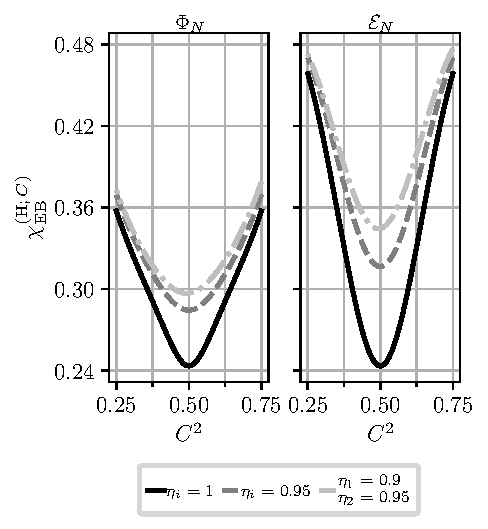
\includegraphics[height=.225\textheight]{pics/homodyne/chi_cf.pdf}
\caption[]{}
\label{subfig:h-cf-a}
        \end{subfigure}
        \hfill
        \begin{subfigure}[c]{.3\linewidth}
          \centering
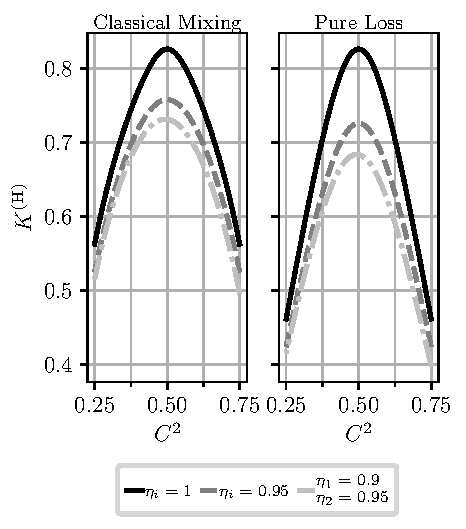
\includegraphics[height=.225\textheight]{pics/homodyne/r_cf.pdf}
\caption[]{}
\label{subfig:h-cf-b}
        \end{subfigure}
        \hfill
        \begin{subfigure}[c]{.3\linewidth}
          \centering
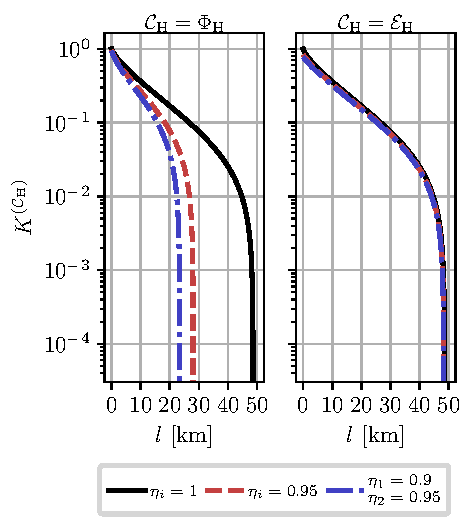
\includegraphics[height=.225\textheight]{pics/homodyne/r(l)_cf.pdf}
\caption[]{}
\label{subfig:h-cf-c}
        \end{subfigure}
        \caption{
        (a)~Holevo information, $\chi_{\ind{EB}}^{(C_{\ind{H}})}$ and (b)~asymptotic secret fraction, $K^{(C_{\ind{H}})}$, as a function of the beam splitter transmission, $C^2$, of the homodyne receiver computed at different values of
        the detector efficiencies for additive-noise and attenuator channel models, as indicated in panel title.
        The parameters are: $V = 5;\, T_{\ind{ch}} = 0.95;\, \xi_{\ind{ch}} = 10^{-2};$ and $\beta = 0.95$.    
        (c)~$K^{(C_{\ind{H}})}$ versus transmission length $l$ for additive-noise and attenuator channel models.
        The parameters are:
        $V=5$;\, $\beta=0.95$;\, $\xi_{\ind{ch}}=10^{-2};$ losses are $20$ dB per $100$ km.}
        \label{fig:h-comparison-CM}
\end{figure}
\subsection{Homodyne detection}
For attenuator channel, from Eq.~\eqref{eq:psi_action} and~\eqref{eq:cos-theta-h} we have
\begin{align}
    \label{eq:psi-h-action}
    &\Sigma_{\ind{AB}}^{(\mathcal{E}_{\ind{H}})}=
    \begin{pmatrix}
        V\mathbbm{1}&\frac{c}{\sqrt{\sigma_x}}\sigma_z\\
        \frac{c}{\sqrt{\sigma_x}}\sigma_z&\frac{1}{{\sigma_x}}\left(V_{\ind{B}}+\sigma_N\right)\mathbbm{1}
    \end{pmatrix}\equiv
    \begin{pmatrix}
        V\mathbbm{1}&\tilde{c}\sigma_z\\
        \tilde{c}\sigma_z&\tilde{V}_{\ind{B}}\mathbbm{1}
    \end{pmatrix},\\
    &\tilde{V}_{\ind{B}}\equiv
    {T}(V-1)+1+{\xi}
    ,\\
    &\tilde{c}\equiv\sqrt{{T}(V^2-1)},
\end{align}
where we defined scaled Bob's variance and scaled correlations between Alice and Bob $\tilde{V}_{\ind{B}}$ and $\tilde{c}$, using total channel transmission ${T}$ that consists of channel transmission $T_{\ind{ch}}$ and detection losses $\frac{1}{\sigma_x}$, as well as scaled noise variance $\xi$,
\begin{subequations}
\label{eq:tot_hom}
\begin{align}
    \label{eq:T_tot_hom}
    &T=T_{\ind{ch}}\cdot \frac{1}{\sigma_x},\\
    \label{eq:xi_tot_hom}
    &\xi\equiv\xi_{\ind{ch}}\cdot\frac{1}{\sigma_x}.
\end{align}
\end{subequations}

It follows that for homodyne detection the effect of measurement asymmetry is equivalent to scaling both channel transmission~\eqref{eq:T_tot_hom} and channel noise~\eqref{eq:xi_tot_hom} by a factor of $\sigma_x^{-1}$.

Symplectic eigenvalues of $\Sigma_{\ind{AB}}^{(\mathcal{E}_{\ind{H}})}$, $\nu_{1,2}^{(\mathcal{E}_{\ind{H}})}$, can be computed using formulas~\cite{Weed:rmp:2012}:
\begin{align}
    \label{eq:lambda12-h}
    \nu_{1,2}^{(\mathcal{E}_{\ind{H}})}=\frac{z\pm[\tilde{V}_{\ind{B}}-V]}2,\quad z=\sqrt{\left(V+\tilde{V}_{\ind{B}}\right)^2-4{\tilde{c}^2}},
\end{align}
and then substitued in Eq.~\eqref{eq:S_AB-gamma} to calculate joint entropy $S_{\ind{AB}}^{(\mathcal{E}_{\ind{H}})}$.

Fig.~\ref{fig:h-comparison-CM} illustrates the effects of homodyne measurement asymmetry on Holevo information~\eqref{eq:chi} and asymptotic secret fraction~\eqref{eq:r} versus beam splitter transmission $C^2$, as well as secret fraction versus transmission length, for both additive-noise~\eqref{eq:sigma_m_cov} and attenuator~\eqref{eq:psi_action} channels.
While channel noise is reduced in this setup~\eqref{eq:xi_tot_hom}, so is channel transmission~\eqref{eq:T_tot_hom}, and, since transmission is scaled by modulation variance $V\gg1$ in every expression, as well as reduced mutual information with greater asymmetry per Eq.~\eqref{eq:I_H_res}, attenuator channel has negative effect. 
As shown in Fig.~\ref{subfig:h-cf-a} and~\ref{subfig:h-cf-b}, the attenuator channel results in higher Holevo information, and thus lower secret fraction, at high transmission for fixed asymmetry parameters. However, Fig.~\ref{subfig:h-cf-c} reveals that the attenuator channel achieves significantly greater reach (maximum transmission length at which a positive key rate is obtained) than the additive-noise channel.

\subsection{Double-homodyne detection}
\begin{figure}[t]
    \centering
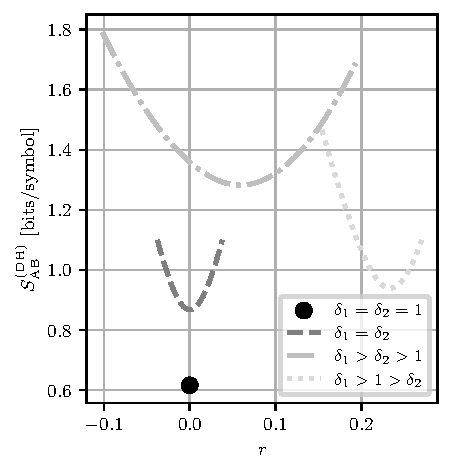
\includegraphics[]{pics/double-homodyne/Sab.pdf}
 \caption[]{Holevo information, $\chi_{\ind{EB}}^{(\ind{DH}; C_{\ind{DH}})}$, as a function of the squeezing parameter $r$ at
    different values of $\delta_{1,2}$. Black dot corresponds to the case of perfect measurements.
    Solid and dashdotted curves correspond to additive-noise channel model, while dashed and dotted curves are for attenuator channel model.
    Color-matched white-filled dots mark points where Holevo information is undefined at the boundaries of the $r$ interval~\eqref{eq:r1-r2} (see Eq.~\eqref{eq:a_def} and main text).
    Values of $\delta_{1,2}$ are: $\delta_{1,2}=1.1$ for solid and dashed curves, $\delta_1=1.75, \delta_2=1.25$ for dashdotted and dotted curves.
    The channel parameters are: $V=5$; $T_{\ind{ch}}=0.95$; and
    $\xi_{\ind{ch}}=10^{-2}$.}
  \label{fig:Entropy}
\end{figure}

For attenuator channel, from Eq.~\eqref{eq:psi_action} and~\eqref{eq:cos-theta-dh} we have
\begin{align}
    &\Sigma_{\ind{AB}}^{(\mathcal{E}_{\ind{DH}})}=
    \begin{pmatrix}
        V\mathbbm{1}&{c}\cos\theta_{\ind{DH}}\sigma_z\\
        c\cos\theta_{\ind{DH}}\sigma_z&
        \begin{matrix}
      \cos^2\theta_{\ind{DH}}\left({V_{\ind{B}}}+\delta_1-\frac{e^{2r}}{\cos^2\theta_{\ind{DH}}}\right)&0\\
      0&\cos^2\theta_{\ind{DH}}\left({V_{\ind{B}}}+\delta_2-\frac{e^{-2r}}{\cos^2\theta_{\ind{DH}}}\right)
    \end{matrix}
    \end{pmatrix}
    \end{align}

Symplectic eigenvalues of this matrix can be calculated using invariants similarly to Eq.~\eqref{eq:nu-12-gamma}. It is obvious that these symplectic eigenvalues, and thereby joint entropy, is explicitly depended on squeezing parameter $r$~\eqref{eq:r1-r2}, like in the case of additive-noise channel (see Ref.~\cite{naumchik2025asymmetryeffectshomodyneheterodyne}). 

Fig.~\ref{fig:Entropy} illustrates dependence of Holevo information on the squeezing parameter, for both additive-noise and attenuator channels. Referring to Fig.~\ref{fig:Entropy}, in the limiting case of ideal double-homodyne detection with $\delta_1=\delta_2=1$, only one value of $r=0$ is allowed (see Ref.~\cite{naumchik2025asymmetryeffectshomodyneheterodyne}), with equal values of Holevo information for both channels (black dot on plot).

When $\delta_1=\delta_2>1$, dependence of Holevo information on squeezing parameter is symmetrical around $r=0$ for both channels. For additive-noise channel, $r=0$ is the point of maximal Holevo information, while for attenuator channel $r=0$ corresponds to minimal Holevo information. Moreover, while Holevo information is unidefined at $r=r_{2,1}$ (see Eq.~\eqref{eq:cos-theta-dh}), the values tend to the same values of joint entropy in the case of additive-noise channel, as signified by color-matched white-filled dots in Fig.~\ref{fig:Entropy}.

For the asymmetric parameter sets considered, where $\delta_1\neq\delta_2$, the Holevo information for both channel models becomes asymmetric about its extrema, resulting in unequal joint entropies at $r=r_{2,1}$. For these parameter sets, the Holevo information is concave in $r$ for the additive-noise channel and convex in $r$ for the attenuator channel.

\begin{figure}[htb]
        \centering
        \begin{subfigure}[c]{.45\linewidth}
            \centering
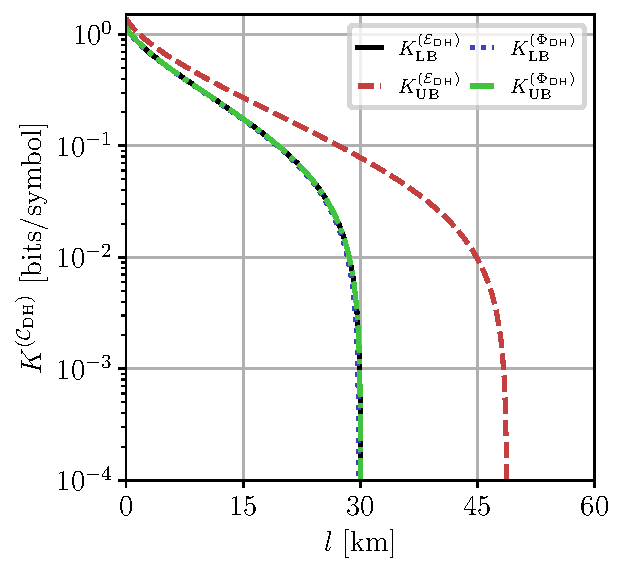
\includegraphics[width=\linewidth]{pics/double-homodyne/1.0.pdf}
\caption[]{$q=1$}
\label{subfig:K-vs-L-q-add-a}
        \end{subfigure}
        \hfill
        \begin{subfigure}[c]{.45\linewidth}
            \centering
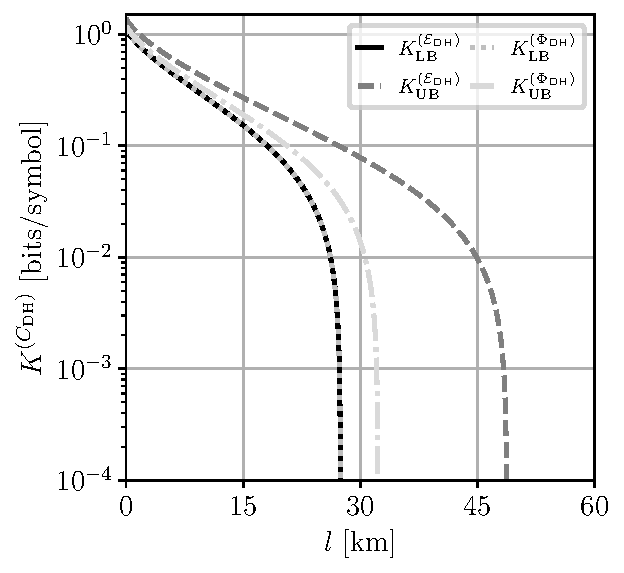
\includegraphics[width=\linewidth]{pics/double-homodyne/1.25.pdf}
\caption[]{$q=1.25$}
\label{subfig:K-vs-L-q-add-b}
        \end{subfigure}
        \caption{Asymptotic secret fraction $K^{(C_{\ind{DH}})}$ versus channel length $l$, computed for fixed $\sigma_x^{(i)}=1.05$ (see Eq.\eqref{eq:sigm-x-i}) and various imbalance ratios $q\equiv\frac{S_S^2}{C_S^2}$ for additive-noise and attenuator channel models (see Fig.~\ref{fig:Entropy}).
        The parameters are:
        $V=5$; $\beta=0.95$; $\xi_{\ind{ch}}=10^{-2};$ losses are $20$ dB per $100$ km.}
        \label{fig:K-vs-L-q-add}
\end{figure}

Fig.~\ref{fig:K-vs-L-q-add} illustrates lower and upper bounds of the asymptotic secret fraction versus transmission length, for both additive-noise~\eqref{eq:sigma_m_cov} and attenuator~\eqref{eq:psi_action} channels. Note that for chosen $\sigma_x^{(i)}$ lower bounds for both channels coincide, because for $\sigma_x^{(i)}\approx1$ maximum of joint entropy for both models is either at $r=r_1$ or $r=r_2$. Moreover, the upper bound for additive-noise channel in Fig.~\ref{subfig:K-vs-L-q-add-a} is very close (0.2 km difference) to the lower bound. 

As seen from Fig.~\ref{fig:K-vs-L-q-add}, difference between lower and upper bound of the asymptotic secret fraction is greater in 

\begin{figure}[htb]
    \centering
        \begin{subfigure}[c]{.3\linewidth}
          \centering
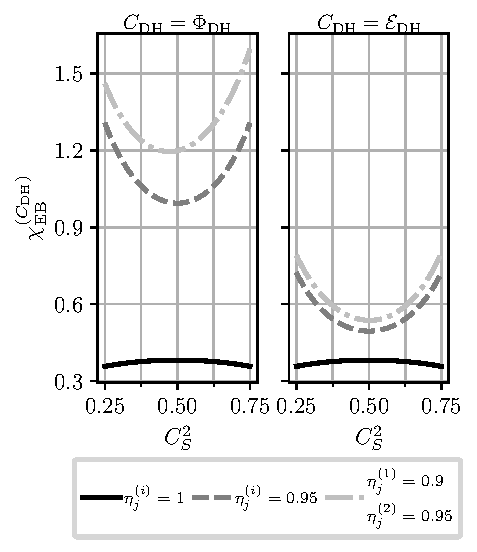
\includegraphics[height=.25\textheight]{pics/double-homodyne/chi_cf.pdf}
\caption[]{}
\label{subfig:dh-cf-a}
        \end{subfigure}
        \hfill
        \begin{subfigure}[c]{.3\linewidth}
          \centering
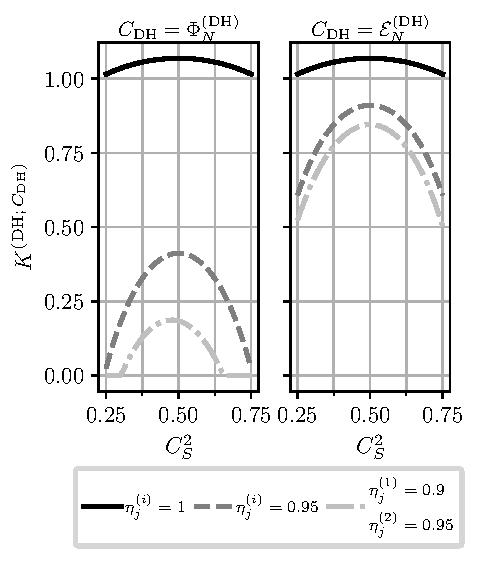
\includegraphics[height=.25\textheight]{pics/double-homodyne/r_cf.pdf}
\caption[]{}
\label{subfig:dh-cf-b}
        \end{subfigure}
        \hfill
        \begin{subfigure}[c]{.3\linewidth}
          \centering
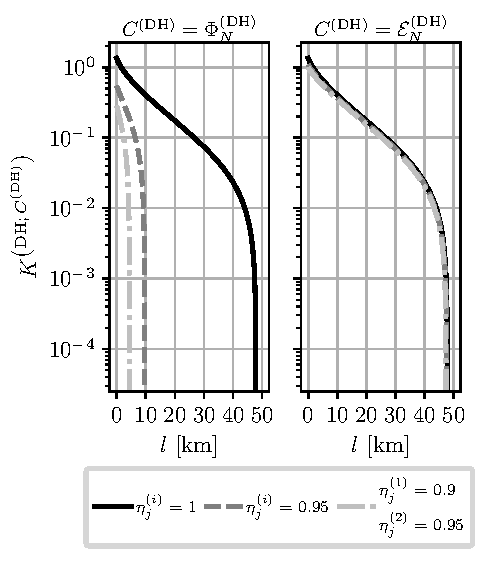
\includegraphics[height=.25\textheight]{pics/double-homodyne/r(l)_cf.pdf}
\caption[]{}
\label{subfig:dh-cf-c}
        \end{subfigure}
        \caption{
        (a)~Holevo information, $\chi_{\ind{EB}}^{(C_{\ind{DH}})}$ and (b)~asymptotic secret fraction, $K^{(C_{\ind{DH}})}$, as a function of the signal beam splitter transmission, $C_S^2$, of the double-homodyne receiver computed at different values of
        the detector efficiencies for additive-noise and attenuator channel models, as indicated in panel title.
        The parameters are: $V = 5; \,T_{\ind{ch}} = 0.95; \,\xi_{\ind{ch}} = 10^{-2};$ and $\beta = 0.95$.    
        (c)~$K^{(C_{\ind{DH}})}$ versus transmission length $l$ for additive-noise and attenuator channel models. 
        The parameters are:
        $V=5$; $\beta=0.95$; $\xi_{\ind{ch}}=10^{-2};$ losses are $20$ dB per $100$ km..
        For both channel models $r=\frac{r_2+r_1}{2}$ (see main text).}
        \label{fig:dh-comparison-CM}
\end{figure}

Fig.~\ref{fig:dh-comparison-CM} illustrates the dependence of Holevo information~\eqref{eq:chi} and asymptotic secret fraction~\eqref{eq:r} on the signal beam splitter transmission $C_S^2$, as well as secret fraction versus transmission length if the receiver uses double-homodyne detection, for both additive-noise~\eqref{eq:sigma_m_cov} and attenuator~\eqref{eq:psi_action} channels.
Unlike the homodyne detection case (see Fig.~\ref{fig:h-comparison-CM}), Holevo information is significantly lower for attenuator channel, except for the ideal measurements case ($\eta_{1,2}^{(1,2)}=1$ and whole $C_S^2$ axis, unlike in homodyne case where ideal measurements are strictly $\eta_{1,2}=1$ and $C^2=0.5$) as both channels have no effect and thereby have equal joint entropies (black curve).
High difference in Holevo information is due to the dependence of joint entropy on $r$ (see Fig.~\ref{fig:Entropy}) and fixing $r=\frac{r_2+r_1}{2}$ for both curves, effectively minimizing Holevo information for attenuator channel and maximizing it for additive-noise channel. 

Analogously to the case of homodyne detection (see Fig.~\ref{subfig:h-cf-c}), in the case of double-homodyne detection the attenuator channel has greater reach than the additive-noise channel, as illustrated by Fig.~\ref{subfig:dh-cf-c}.

%\printbibliography
\section{Discussion and conclusion}
\label{sec:conclusion}

In this paper, we have constructed and compared additive-noise and
attenuator channel representations of noisy homodyne and
double-homodyne measurements affected by receiver asymmetry. Our approach requires the dual of the selected Gaussian channel, together with a
deterministic invertible rescaling of the measurement outcomes, to
reproduce the target noisy Gaussian measurement. At the level of covariance matrices, this condition is expressed by
Eq.~\eqref{eq:C-gen}. These conditions constrain the channel parameters; under the assumptions adopted here, the parameters are then determined by the receiver parameters and, for double-homodyne detection, by $r$.


After the deterministic invertible rescaling of the measurement
outcomes, the two channels reproduce the same conditional
statistics of Bob's outcomes. They therefore give the same Alice-Bob mutual information.
For fixed source and channel parameters, the conditional
covariance matrix in Eq.~\eqref{eq:serf-a|b}, and hence the conditional
entropy $S_{A|B}^{(\gamma)}$, are the same for the two channels because the
detector imperfections enter the conditional state through the same
noisy measurement. The difference between the security estimates originates from the joint state of Alice and Bob. The additive-noise and attenuator channels generally produce different joint covariance matrices and, consequently, different joint entropies. In the untrusted-detector model considered in this paper, the environmental output of the selected channel is assigned to Eve. The corresponding Holevo information~\eqref{eq:chi} therefore depends on the selected channel even when Bob's observed statistics remain unchanged.


For homodyne detection, we take the environmental mode of the attenuator channel to be in the
vacuum state, so that the detector imperfections are represented by a
pure-loss channel. This
channel rescales both the effective transmission and the
output-referred excess noise by the same factor, as shown in
Eq.~\eqref{eq:tot_hom}.

The numerical results in Fig.~\ref{fig:h-comparison-CM} show that the additive-noise and
attenuator channels give significantly different security estimates. At high channel
transmittance and for the parameters considered, the attenuator
channel gives a larger Holevo information and a lower asymptotic
secret fraction. At longer distances, however, the secret fraction remains positive up
to a greater channel length than in the additive-noise channel. Therefore, neither channel can be described as
strictly more or less pessimistic.

A distinguishing feature of double-homodyne detection is the
nonuniqueness of the representation of its noisy POVM. The covariance
matrix of the physical double-homodyne measurement is fixed
by the receiver parameters and does not depend on the squeezing
parameter $r$. The effects of the ideal Gaussian POVM are proportional to projectors onto displaced squeezed states and depend on $r$. The noisy POVM is obtained by applying the dual of the selected Gaussian channel to the ideal POVM, together with the outcome rescaling. The requirement that the excess-noise covariance matrix be positive
semidefinite restricts $r$ to the interval given by
Eq.~\eqref{eq:r1-r2}.

For the additive-noise channel, variation of $r$ redistributes the
measurement noise between the two conjugate quadratures according to
Eq.~\eqref{eq:sigma_N-sq-2}. For the attenuator channel, the same variation changes
both the attenuation coefficient and
the covariance matrix of the environmental state, as described by
Eqs.~\eqref{eq:cos-theta-dh} and~\eqref{eq:a_def}. In the attenuator channel considered here, the generally anisotropic
measurement noise is reproduced by an environmental mode in an anisotropic Gaussian
state, which was chosen to be pure.

At the boundaries of the admissible interval of the squeezing parameter
$r$, one of the additive-noise quadrature variances vanishes. In the
attenuator channel, the environmental state approaches an
infinitely squeezed limit: one quadrature variance tends to zero,
whereas the conjugate variance diverges. The boundary points are
therefore understood as limiting channels in which the attenuator
result approaches the corresponding additive-noise result.

Figure~\ref{fig:Entropy} shows that the Holevo information depends on
$r$ in qualitatively different ways for the two channel models.
For the parameter sets considered, this dependence is concave for
the additive-noise channel and convex for the attenuator
channel. When the measurement noise is symmetric between the two
quadratures, both curves are symmetric about $r=0$. In this case, the coherent state, given by $r=0$, maximizes the Holevo
information for the additive-noise channel and minimizes it for the
attenuator channel.
For the asymmetric case considered, this symmetry is lost and the
extrema are shifted away from $r=0$.

The lower and upper secret-fraction curves in Fig.~\ref{fig:K-vs-L-q-add} describe the range
obtained by varying $r$ over its admissible interval for each channel model. For the near-ideal quadrature variances used in
Fig.~\ref{fig:K-vs-L-q-add}, the lower bounds of the two channels nearly coincide
because the Holevo-information maximum occurs at, or close to, the
interval boundaries. The upper bounds become more clearly separated
when the imbalance of the signal beam splitter is increased.

The comparison shown in Fig.~\ref{fig:dh-comparison-CM} was performed at
the midpoint of the admissible interval of $r$. In the symmetric case, this value coincides with the
maximum of the additive-noise Holevo information and the minimum of
the attenuator Holevo information. The pronounced separation between
the secret fractions in Fig.~\ref{fig:dh-comparison-CM} therefore reflects both the selected
channel model and the selected squeezing parameter.

These results clarify the role of the chosen channel representation when receiver noise is treated as untrusted. Although the additive-noise and attenuator channels reproduce the same receiver statistics after outcome rescaling, they generally yield different joint states of Alice and Bob and different environmental outputs assigned to Eve. Choosing a particular channel representation therefore introduces a physical assumption about the coupling between the optical signal and the inaccessible degrees of freedom.
A security estimate should not be based on a particular channel representation solely because it gives a larger secret fraction. The selected representation should either be justified from the physical structure of the receiver or the dependence of the estimate on the channels included in the analysis should be reported explicitly. The present comparison is restricted to the additive-noise channel and to attenuator channels whose environmental modes are in pure Gaussian states. Mixed environmental states and other Gaussian channel representations compatible with the same receiver statistics were not considered.

Appendix~\ref{sec:lossy-bs} extends the receiver model to include
independent pure losses at the output ports of a lossless beam splitter.
These losses can be incorporated into the effective photodetector
efficiencies. By contrast, a general lossy asymmetric beam splitter
with unequal complex transmission and reflection amplitudes does not,
in general, preserve the simple quadrature form of the receiver
response and cannot be included by merely replacing the detector
efficiencies.

The security analysis was performed in the asymptotic limit for the GMCS CV-QKD protocol under collective Gaussian attacks,
with the modeled receiver imperfections treated within an untrusted-detector model. Trusted receiver noise,
finite-size corrections, active detector attacks, and uncertainties in
the calibration parameters require separate treatment. Within these
assumptions, equivalent receiver statistics can lead to different
estimates of Eve's information when different channel representations are used within the untrusted-detector model.

%%%%%%%%%%%%%%%%%%%%%%%%%%%%%%
\section*{Acknowledgements}
The work was supported by the Russian Science Foundation (project No. \textcolor{red}{24-11-00398}).
%%%%%%%%%%%%%%%%%%%%%%%%%%%%%%%%%

\appendix
\section{Lossy beam splitter}
\label{sec:lossy-bs}
In this appendix, %we discuss how the formulas describing homodyne and double-homodyne detection cases relate to the case if beam splitters are lossy.
we show that applying independent pure loss channels at the output ports of a lossless beam splitter yields the exact same transformation as a single formally defined lossy beam splitter.

First, consider the case of homodyne detection.
The lossless unbalanced beam splitter mixes the input signal mode $\hat{a}$ and the local oscillator mode $\hat{a}_L$. This transformation is described by the unitary rotation matrix $\vc{U}_{\ind{BS}}$,
\begin{align}
    \begin{pmatrix}
        \hat a_{1}\\
        \hat a_{2}
    \end{pmatrix}
    &=
    \vc{U}_{\ind{BS}}
    \begin{pmatrix}
        \hat a\\
        \hat a_{L}
    \end{pmatrix}
    =
    \begin{pmatrix}
        C & S \\
        -S & C
    \end{pmatrix}
    \begin{pmatrix}
        \hat a\\
        \hat a_{L}
    \end{pmatrix}
    \nonumber\\
    &=
    \begin{pmatrix}
        C\hat{a}+S\hat{a}_L\\
        -S\hat{a}+C\hat{a}_L
    \end{pmatrix},
\end{align}
where $C$ and $S$ are the transmission and reflection coefficients of the beam splitter BS, respectively.

We model the subsequent losses by passing each intermediate output mode $\hat{a}_{1,2}$ through a virtual beam splitter of transmittance $\tau_{1,2}$. This mixes each signal with an independent environmental vacuum mode $\hat{v}_{1,2}$, where $[\hat{v}_i, \hat{v}_j^\dag] = \delta_{ij}$,
\begin{align}
    \begin{pmatrix}
        \hat b_{1}\\
        \hat c_{1}
    \end{pmatrix}&=
    \begin{pmatrix}
        \sqrt{\tau_1}&-\sqrt{1-\tau_1}\\\sqrt{1-\tau_1}&\sqrt{\tau_1}
    \end{pmatrix}
    \begin{pmatrix}
        \hat a_1\\
        \hat v_1
    \end{pmatrix},\\
    \begin{pmatrix}
        \hat b_{2}\\
        \hat c_{2}
    \end{pmatrix}&=
    \begin{pmatrix}
        \sqrt{\tau_2}&-\sqrt{1-\tau_2}\\\sqrt{1-\tau_2}&\sqrt{\tau_2}
    \end{pmatrix}
    \begin{pmatrix}
        \hat a_2\\
        \hat v_2
    \end{pmatrix}.
\end{align}
Tracing out the lost environmental modes $\hat{c}_{1,2}$, the remaining physical output modes $\hat{b}_{1,2}$ expand to
\begin{align}
    \label{eq:b1b2-out}
    \begin{pmatrix}
        \hat b_{1}\\
        \hat b_{2}
    \end{pmatrix}
    =
    \begin{pmatrix}
        \sqrt{\tau_1}C & \sqrt{\tau_1}S\\
        -\sqrt{\tau_2}S & \sqrt{\tau_2}C
    \end{pmatrix}
    \begin{pmatrix}
        \hat{a}\\
        \hat{a}_L
    \end{pmatrix}
    +
    \begin{pmatrix}
        -\sqrt{1-\tau_1}\hat{v}_1\\
        -\sqrt{1-\tau_2}\hat{v}_2
    \end{pmatrix}.
\end{align}
From Eq.~\eqref{eq:b1b2-out}, we extract the effective scattering matrix $\vc{T}_{\ind{BS}}$ and the fluctuation noise operators $\hat{F}_{1,2}$ representing the device excitations
\begin{align}
    \label{eq:T_eff_extract}
    \vc{T}_{\ind{BS}}
    =
    \begin{pmatrix}
        \sqrt{\tau_1}C & \sqrt{\tau_1}S\\
        -\sqrt{\tau_2}S & \sqrt{\tau_2}C
    \end{pmatrix}.
\end{align}

It is not difficult to show that to preserve the Canonical Commutation Relations for the output fields, $[\hat{b}_i, \hat{b}_j^\dagger] = \delta_{ij}$, the noise operators $\hat{F}_{1,2}$ must satisfy
\begin{align}
  [\hat F_i, \hat F_j^\dagger] = \delta_{ij} - \sum_{k} T_{ik} T_{jk}^*,
\end{align}
where $T_{ik}$ are the elements of the scattering matrix $\vc{T}_{\ind{BS}}$~\eqref{eq:T_eff_extract}.
Evaluating this constraint explicitly using the elements of $\vc{T}_{\ind{BS}}$ yields:
\begin{align}
    &[\hat F_1, \hat F_1^\dagger] = %1 - |T_{11}|^2 - |T_{12}|^2 = 1-\tau_1 C^2-\tau_1 S^2 = 
    1-\tau_1,\\
    &[\hat F_2, \hat F_2^\dagger] = %1 - |T_{21}|^2 - |T_{22}|^2 = 1-\tau_2 S^2-\tau_2 C^2 = 
    1-\tau_2,\\
    &[\hat F_1, \hat F_2^\dagger] = %0 - (T_{11}T_{21}^* + T_{12}T_{22}^*) = -\left[(\sqrt{\tau_1}C)(\sqrt{\tau_2}S) + (-\sqrt{\tau_1}S)(\sqrt{\tau_2}C)\right] = 
    0,
\end{align}
which matches the commutators calculated from Eq.~\eqref{eq:b1b2-out}.


We now connect this setup to the formal, standard mathematical treatment of lossy beam splitters~\cite{Barnett1998,Knll1999}. This framework models loss via an interaction matrix $\vc{A}$ acting on ancillary modes, which must obey the positivity condition $\vc{1}-\vc{A}\hcnj{\vc{A}}\ge 0$ to satisfy unitarity. Note that the extracted scattering matrix $\vc{T}_{\ind{BS}}$~\eqref{eq:T_eff_extract} can be factored into a product of a diagonal scaling matrix and the lossless unitary,
\begin{align}
    \label{eq:R_eff}
    \vc{T}_{\ind{BS}}
    &=
    \begin{pmatrix}
        \sqrt{\tau_1} & 0\\
        0 & \sqrt{\tau_2}
    \end{pmatrix}
    \begin{pmatrix}
        C & S\\
        -S & C
    \end{pmatrix}
    \nonumber\\
    &=
    \begin{pmatrix}
        \sqrt{\tau_1} & 0\\
        0 & \sqrt{\tau_2}
    \end{pmatrix}
    \vc{U}_{\ind{BS}}.
\end{align}
By defining the positive semi-definite matrix representing the loss properties as $\vc{A}\hcnj{\vc{A}}=\diag(1-\tau_1,1-\tau_2)$, it follows that:
\begin{align}
    \sqrt{\vc{1}-\vc{A}\hcnj{\vc{A}}} = \begin{pmatrix} \sqrt{\tau_1} & 0 \\\\ 0 & \sqrt{\tau_2} \end{pmatrix}.
\end{align}
Substituting this back into Eq.~\eqref{eq:R_eff} yields the polar decomposition of the scattering matrix of a lossy beam splitter in its generalized form~\cite{Knll1999}:
\begin{align}
  \label{eq:lossy-T}
  \vc{T}_{\ind{BS}}=\sqrt{\vc{1}-\vc{A}\hcnj{\vc{A}}}\,\vc{U}_{\ind{BS}}.
\end{align}
Because the matrix $\vc{A}\hcnj{\vc{A}}$ representing the losses is diagonal, it is straightforward to see that to account for lossy beam splitter in a homodyne setup it is sufficient to simply rescale the quantum efficiencies of detection: $\eta_{1,2}\to\tau_{1,2}\eta_{1,2}$. The same argument would apply in the case of double-homodyne detection.

We conclude this appendix by discussing the generalized (asymmetrical) beam splitter model where input ports of the beam splitter are characterized by different set of transmission and reflection coefficients. In this case, the non-unitary scattering matrix is written in the form~\cite{Uppu_2016}
\begin{align}
  \vc{S}
  =
  \begin{pmatrix}
    t & \rho\\
    r & \tau
  \end{pmatrix},
  \qquad
  \vc{S}\hcnj{\vc{S}}\leq\vc{1},
\end{align}
where $t, \tau$ ($r, \rho$) are complex transmission (reflection) coefficients.%, and $\phi_{1,2}$ are the phase shifts. 
While it can be factored into lossy and unitary parts similarly to~\eqref{eq:lossy-T}, \textcolor{red}{this case cannot be covered by the formulas after some replacement, because it ruins quadrature representation:}
\begin{align}
  %\label{eq:BS}
  &
    \ket{\alpha,\alpha_L}\mapsto\ket{\alpha_1,\alpha_2},
  \\
  &
    %\label{eq:amplitudes}
    \alpha_1=t\alpha+\rho \alpha_L,\quad
    \alpha_2=r\alpha+\tau\alpha_L,
\end{align}

\begin{align}
  &
  %\label{eq:Gaussian}
    \prob_G(\mu)=G(\mu-\mu_G;\sigma_G),
    \\
    \label{eq:sigma_G-general-lossy-bs}
    \sigma_G
    &=
    \eta_1|\alpha_1|^2+\eta_2|\alpha_2|^2
    \nonumber\\
    &=
    \left(
        \eta_1|\rho|^2+\eta_2|\tau|^2
    \right)|\alpha_L|^2
    +
    \left(
        \eta_1|t|^2+\eta_2|r|^2
    \right)|\alpha|^2
    \nonumber\\
    &\quad
    +
    2\operatorname{Re}
    \left[
        \left(
            \eta_1t\rho^*
            +
            \eta_2r\tau^*
        \right)
        \alpha\alpha_L^*
    \right]
    \nonumber\\
    &\approx
    \left(
        \eta_1|\rho|^2+\eta_2|\tau|^2
    \right)|\alpha_L|^2
    +
    2\operatorname{Re}
    \left[
        \left(
            \eta_1t\rho^*
            +
            \eta_2r\tau^*
        \right)
        \alpha\alpha_L^*
    \right],
    \\
    \label{eq:mu_G-general-lossy-bs}
    \mu_G
    &=
    \eta_1|\alpha_1|^2-\eta_2|\alpha_2|^2
    \nonumber\\
    &=
    \left(
        \eta_1|\rho|^2-\eta_2|\tau|^2
    \right)|\alpha_L|^2
    +
    \left(
        \eta_1|t|^2-\eta_2|r|^2
    \right)|\alpha|^2
    \nonumber\\
    &\quad
    +
    2\operatorname{Re}
    \left[
        \left(
            \eta_1t\rho^*
            -
            \eta_2r\tau^*
        \right)
        \alpha\alpha_L^*
    \right]
    \nonumber\\
    &\approx
    \left(
        \eta_1|\rho|^2-\eta_2|\tau|^2
    \right)|\alpha_L|^2
    +
    2\operatorname{Re}
    \left[
        \left(
            \eta_1t\rho^*
            -
            \eta_2r\tau^*
        \right)
        \alpha\alpha_L^*
    \right].
\end{align}

\section{Fluctuating Local Oscillator} \label{sec:fluc-LO}
In this Appendix, we extend the theoretical treatment of homodyne measurements to account for classical intensity fluctuations of the local oscillator (LO).% In the main text, the LO amplitude $\vert\alpha_L\vert$ is treated as a fixed constant. Here, we model it as a fluctuating quantity and evaluate its impact on the Gaussian-approximated POVM.

We start from the Gaussian approximation of the photon count difference probability distribution in homodyne scheme~\cite{naumchik2025asymmetryeffectshomodyneheterodyne}
\begin{align}
  &
  \label{eq:Gaussian}
    \prob_G(\mu)=G(\mu-\mu_G;\sigma_G),
    \\
  &
    \label{eq:sigma_G}
    \sigma_G=\eta_1|\alpha_1|^2+\eta_2|\alpha_2|^2
    \approx
    (\eta_1S^2+\eta_2C^2) \left|\alpha_L\right|^2,
  \\
  &
    \label{eq:mu_G}
    \mu_G=\eta_1|\alpha_1|^2-\eta_2|\alpha_2|^2
    \approx
    (\eta_1S^2-\eta_2C^2) \left|\alpha_L\right|^2
    +CS (\eta_1+\eta_2) \left|\alpha_L\right| \avr{\hat{x}_\phi},
\end{align}
where
\begin{align}
      \label{eq:G-notation}
    G(x;\sigma)\equiv\frac{1}{\sqrt{2\pi\sigma}}\exp\Bigl(-\frac{x^2}{2\sigma}\Bigr).
\end{align}

We assume that the LO amplitude fluctuates around its mean value $\alpha_L$ such that
\begin{align}
\alpha_L = \alpha_L + \delta \alpha_L, \quad \delta \alpha_L \sim G(\delta \alpha_L, \sigma_{L})
\end{align}
where $\sigma_{LO}$ represents the variance of the LO amplitude fluctuations.

To find the total probability distribution $\prob_{\ind{tot}}(\mu)$ that accounts for the local oscillator fluctuations, we perform an ensemble average by integrating the conditional distribution $\prob_G(\mu)$ over the Gaussian prior of the LO amplitude.% We assume the phase $\phi = \arg\alpha_L$ is locked, so that the amplitude fluctiation $\delta\alpha_L$ is real-valued random variable. 
\begin{align}
    \label{eq:average-integral}
    \prob_{\text{total}}(\mu) = \int \mathop{\dd\delta \alpha_L} \prob_G(\mu \vert \delta\alpha_L) \prob_G(\delta\alpha_L) =
    %\int_{-\infty}^{\infty} \mathop{\dd\delta \alpha_L} G\left(\mu - \mu_G - \frac{\partial \mu_G}{\partial \left|\alpha_L\right|} \delta\alpha_L; \sigma_G\right) G(\delta\alpha_L; \sigma_L),
\end{align}
%where the effective  total variance
%\begin{align}
%    \overline{\mu}_G &= (\eta_1S^2-\eta_2C^2) \left|\alpha_L\right|^2 + CS (\eta_1+\eta_2) \left|\alpha_L\right| \avr{\hat{x}_\phi}, \\
%    \overline{\sigma}_G &= (\eta_1S^2+\eta_2C^2) \left|\alpha_L\right|^2 + \left[ 2(\eta_1S^2-\eta_2C^2) \left|\alpha_L\right| + CS (\eta_1+\eta_2) \avr{\hat{x}_\phi} \right]^2 \sigma_L.
%\end{align}

%where $\sigma_G$ and $\mu_G$ denote the nominal parameters evaluated at the mean LO amplitude as defined in Eqs.~\eqref{eq:sigma_G} and \eqref{eq:mu_G}. Here, the conditional distribution's mean is linearized to the first order with respect to $\delta\alpha_L$, while its variance is kept to the zeroth order.

S%ubstituting the explicit Gaussian form \eqref{eq:G-notation} into the integral expression yields:
%\begin{align}
%    \prob_{\text{total}}(\mu) = \frac{1}{2\pi \sqrt{\sigma_G \sigma_L}} \int_{-\infty}^{\infty} \exp\left[ -\frac{\left(\mu - \mu_G - \frac{\partial \mu_G}{\partial \left|\alpha_L\right|} \delta\alpha_L\right)^2}{2\sigma_G} - \frac{(\delta\alpha_L)^2}{2\sigma_L} \right] \mathop{\dd\delta \alpha_L}.
%\end{align}
%Expanding the quadratic form within the exponent and collecting the terms with respect to $\delta\alpha_L$, we obtain:
%\begin{align}
%    -\frac{1}{2} \left[ \left( \frac{1}{\sigma_G}\left(\frac{\partial \mu_G}{\partial \left|\alpha_L\right|}\right)^2 + \frac{1}{\sigma_L} \right) (\delta\alpha_L)^2 - 2\frac{\frac{\partial \mu_G}{\partial \left|\alpha_L\right|}(\mu - \mu_G)}{\sigma_G} \delta\alpha_L + \frac{(\mu - \mu_G)^2}{\sigma_G} \right].
%\end{align}
%Completing the square over the integration variable $\delta\alpha_L$ separates the exponent into a shifted quadratic term and a remainder independent of $\delta\alpha_L$:
%\begin{align}
%    -\frac{\left( \delta\alpha_L - \frac{\frac{\partial \mu_G}{\partial \left|\alpha_L\right|} \sigma_L (\mu - \mu_G)}{\sigma_G + \left(\frac{\partial \mu_G}{\partial \left|\alpha_L\right|}\right)^2 \sigma_L} \right)^2}{2 \left( \frac{\sigma_G \sigma_L}{\sigma_G + \left(\frac{\partial \mu_G}{\partial \left|\alpha_L\right|}\right)^2 \sigma_L} \right)} - \frac{(\mu - \mu_G)^2}{2\left( \sigma_G + \left(\frac{\partial \mu_G}{\partial \left|\alpha_L\right|}\right)^2 \sigma_L \right)}.
%\end{align}
%Performing the standard Gaussian integration over $\delta\alpha_L$ cancels out the variable-dependent pre-factors, reducing the total probability distribution directly to:
%\begin{align}
%    \prob_{\text{total}}(\mu) = \frac{1}{\sqrt{2\pi \left[ \sigma_G + \left(\frac{\partial \mu_G}{\partial \left|\alpha_L\right|}\right)^2 \sigma_L \right]}} \exp\left( -\frac{(\mu - \mu_G)^2}{2\left[ \sigma_G + \left(\frac{\partial \mu_G}{\partial \left|\alpha_L\right|}\right)^2 \sigma_L \right]} \right) = G\left(\mu - \mu_G; \sigma_G + \left(\frac{\partial \mu_G}{\partial \left|\alpha_L\right|}\right)^2 \sigma_L \right).
%\end{align}


\bibliography{quant,refs,homodyne,math}

\end{document}
